\documentclass[12pt,titlepage]{article}

\usepackage{graphics}
\usepackage{pdflscape}
\usepackage{array}
\usepackage{color}
\usepackage{colortbl}
\usepackage{xcolor}
\usepackage{url,amsfonts,epsfig}
\usepackage[applemac]{inputenc} %comando per le lettere accentate se usate mac  
%\usepackage[T1]{fontenc}
%\usepackage[utf8]{inputenc}
\usepackage[english]{babel}
%\usepackage[latin1]{inputenc} % comando per le lettere accentate se usate pc  
\usepackage[pagebackref]{hyperref}
\hypersetup{
colorlinks=false,
allbordercolors=white
}

\begin{document}
%Code for title page
\begin{titlepage}
\centering
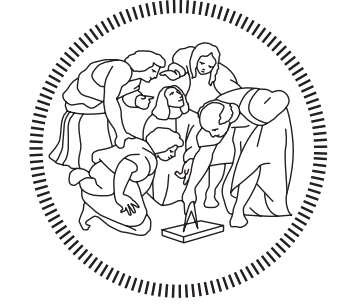
\includegraphics[width=0.4\textwidth]{Logos/LogoPolimi}\par
	{{Politecnico di Milano} \par}
	{{A.A. 2017/2018} \par}
	\vspace{1.5cm}
	
\includegraphics[width=0.9\textwidth]{Logos/LogoTravlendar}\par
	%{\Large{\textsc{{{\color{red}{ \textbf{T}rav}}lendar{\color{red}{+}}}} \\ 
		%Software Engineering 2} \par}f
	\vspace{1.5cm}
	{\Huge \textbf {DD}\par}
	{ \textbf{Design Document} \par}
	\vspace{1.5cm}
	{\Large\itshape Sara Pid\'o  }{\Large   {  894744}\par}
	{\Large\itshape Chiara Plizzari }{\Large   {  893901}\par}
	{\Large\itshape Giuseppe Severino }{\Large   {  898458}\par}
	\vspace{2cm}
	\vfill
	% Bottom of the page
	%{\large Document version: 3.1\par}
\end{titlepage}

\newpage\null\thispagestyle{empty}\newpage

\pagenumbering{roman}

%%%% Opzione per interlinea 2
%%%\baselineskip 18pt

%\maketitle

\tableofcontents
%%\listoffigures
%%\listoftables

\pagebreak

\section{Introduction} \label{introduzione}
\pagenumbering{arabic}
\subsection{Purpose}
With the Design Document we would like to make the idea of Travlendar+ application more precise and more detailed.
In particular the main goal of the DD is  to describe the system in terms of architectural design choices.
It is written in particular for developers to help them to identify the architectural styles, the design patterns, the main components and their interfaces and, last but not least, the runtime behaviour.


\subsection{Scope}

\subsection{Definitions, Acronyms, Abbreviations}
\begin{itemize}
\item DD: design document;
\item RASD: requirements analysis and specification document;
\item API: application programming interface;
\end{itemize}
\subsection{Reference Documents}
\begin{itemize}
\item RASD;
\item Specification Document;
\item Example of DD of previous years;
\end{itemize}
\subsection{Document Structure}
This document is structured as follows:
\paragraph{Section 1: Introduction}
In this section it is described the purpose and the main goals  of the document giving a general description.
\paragraph{Section 2: Architectural Design}
It gives a general view on how the architecture of Travlendar+ should be showing architectural choices, styles and patterns.
\paragraph{Section 3: Algorithm Design}
In this part we include the most critical and relevant parts via algorithms.
\paragraph{Section 4: User Interface Design}
This section provides an overview on how the user will see the application through the mockups and UX and BCE diagrams.
\paragraph{Section 5: Requirements Traceability}
It explains how requirements defined in the RASD must be mapped to the design elements of the application.
\paragraph{Section 6: Implementation, Integration and Test Plan}
This part will include the order of implementation of subcomponents and to integrate them. Moreover it will include our plan to test this integration.
\paragraph{Section 7: Effort spent}
Here are reported the information about the hours of work spent by each member of the group by doing this project.
\paragraph{Section 8: References}

\section{Architectural Design}
\subsection{Overview}
\subsection{Component view}
\subsection{Deployment view}
\subsection{Runtime view}
\subsection{Component interfaces}
\subsection{Selected architectural styles and patterns}
\subsection{Other design decisions}

\section{Algorithm Design}

\section{User Interface Design}

\section{Requirements Traceability}

\section{Implementation, Integration and Test Plan}

\section{Effort Spent}

\section{References}
\end{document}